\documentclass[a4paper, itemph]{oblivoir}
\setmainhangulfont{NANUMMYEONGJO.TTF}[BoldFont={NANUMMYEONGJOEXTRABOLD.TTF}]
\usepackage[english]{babel}
\usepackage[utf8x]{inputenc}
\usepackage[T1]{fontenc}
%% Sets page size and margins
\usepackage[a4paper,top=3cm,bottom=2cm,left=3cm,right=3cm,marginparwidth=2cm]{geometry}

\usepackage{indentfirst}

%% Useful packages
\usepackage{amsfonts}
\usepackage{amsmath, mathtools}
\usepackage{graphicx}
\usepackage{subcaption}
\usepackage[colorinlistoftodos]{todonotes}
\usepackage{amssymb}
\usepackage{amsthm}
\usepackage{tikz}

%Extravaganza
\newtheorem{thm}{Theorem}[subsection]
\newtheorem{lem}{Lemma}[subsection]
\newtheorem{cor}{Corollary}[subsection]
\newcommand{\overbar}[1]{\mkern 1.5mu\overline{\mkern-1.5mu#1\mkern-1.5mu}\mkern 1.5mu}
\theoremstyle{definition}
\newtheorem{defn}{Definition}[subsection]
\newtheorem{rem}{Remark}[subsection]

\begin{document}
\title{기초전자회로 및 실험: Lab \#02}
\author{서울대학교 전기$\cdot$정보공학부 2018-12602 이준협}
\date{April 11, 2020}
\maketitle

\section{Measurements}
\subsection{Half-wave Rectifier}
\begin{table}[htb]
\centering
\begin{tabular}{c|c|c}
    $R$=19.77[k$\Omega$]& Max[V] & Min[V]\\
    \hline
    $V_{in}$(Ch. 2) & 3.88 & -3.96 \\
    \hline
    $V_{out}$(Ch. 1) & 3.16 & -4.00$\times10^{-2}$
\end{tabular}
\caption{Measurement of the half-wave rectifier circuit}
\end{table}

The voltage of the resistor, compared with the input voltage, is seen to be pulled down by $7.2\times10^{-1}$[V] when the input voltage is higher than $7.2\times10^{-1}$[V], and for the rest of the cycle the output stays at $-40$[mV]. The turn on voltage of the diode, therefore, is about $720$[mV], and the reverse bias current is about $-40/19.77=-2.02[\mu$A]. This is considerably different from what was measured in lab 1 as the reverse bias current, which was in the nA range.
\subsection{The Ripple Voltage}
\begin{table}[htb]
    \centering
    \begin{tabular}{c|c|c|c|c|c}
    $C$=0.33[$\mu$F]& Frequency[Hz] & Max[V] & Min[V] & Ripple[V]& $RC\times\mathrm{ln(\dfrac{Max}{Min})}$[ms]\\
    \hline
    $V_{in}$(Ch. 2) & 90 & 4.043 & -3.960 \\
    \hline
    $V_{out}$(Ch. 1) & 90 & 3.480 & 9.422$\times10^{-1}$ & 2.538 & 8.5\\
    \hline
    $V_{in}$(Ch. 2) & 100 & 4.042 & -3.960 \\
    \hline
    $V_{out}$(Ch. 1) & 100 & 3.480 & 1.067 & 2.413 & 7.7\\
    \hline
    $V_{in}$(Ch. 2) & 110 & 4.000 & -4.000\\
    \hline
    $V_{out}$(Ch. 1) & 110 & 3.474 & 1.158 & 2.316 & 7.2
\end{tabular}
    \caption{Measurement of the ripple voltage}
\end{table}

The displayed $V_{d,on}$ is approximately 560[mV], as obtained by calculating the difference between the maximum voltages of $V_{in}$ and $V_{out}$, and the ripple voltage at $f=100$[Hz] is $2.413$[V], which has a 0.542\% error with the desired ripple of 2.4[V]. Therefore, the desired ripple voltage was obtained. Also, the decay time(calculated in the 6th column) and therefore the ripple voltage decreases as the frequency increases, since the input voltage rises faster. Intuitively, this means that the capacitor is given less and less time to charge when the frequency increases.

The time calculated in Table 2 is the time that the voltage decayed($(V_p-V_{d,on})\exp(-t/RC)$) before intersecting with the sinusoidal input pulled down by the diode($V_p\cos(2\pi t/T)-V_{d,on}$), in which the intersection voltage is the peak of the input further pulled down by the ripple voltage($V_p-V_{d,on}-V_R$).
\begin{equation}
V_p\cos{\frac{2\pi t}{T}}-V_{d,on}=(V_p-V_{d,on})\exp\left(-\frac{t}{RC}\right)=V_p-V_R-V_{d,on}
\end{equation}
What we need to confirm is if the constant voltage model holds, i.e if the voltage level given by $V_p\cos{\dfrac{2\pi t}{T}}-V_{d,on}$ is really the minimum voltage of the ripple. However, when we calculate $V_{d,on}$ by the difference between the high voltages of $V_{in}$ and $V_{out}$, the sinusoid voltage actually turns out to be negative; $4.043\cos{(2\pi\times0.0085\times 90)}-(4.043-3.480)=-0.18$[V] in the 90[Hz] range. The reason for this serious error will be explained in the next section.
\section{Comments}
\subsection{Adjusting the Ripple Voltage}

The capacitance to obtain 2.2[V] of ripple voltage is able to be obtained from
\begin{equation}
\frac{RC}{T}=\frac{\left(1-\arccos{\left(1-V_R/V_p\right)}\right)/2\pi}{\mathrm{ln}\left((V_p-V_{d,on})/(V_p-V_{d,on}-V_R)\right)}
\end{equation}
which is equation (1) rearranged. Let $V_p=4$[V], $V_R=2.2$[V], $V_{d,on}=560$[mV](obtained from this experiment), $R=19.77$[k$\Omega$], $T=0.01$[s], then we get $C=0.409$[$\mu$F]. Using standard values, we may use the 0.39[$\mu$F] capacitor.

From equation (2), we can further analyze what happens when parameters are changed.
\subsubsection{When $R, C$ changes}
Note that the right hand side of equation (2) is a decreasing function of $V_R$, the ripple voltage, since the numerator is a decreasing function of $V_R$ and the numerator is an increasing function of $V_R$(-arccos is an increasing function but $V_R$ is inverted in the argument of the numerator, thus it is decreasing). Thus, when $R$ increases, $V_R$ must decrease. Also, identically to the case when $R$ changes, an increase in $C$ corresponds to a decreasing $V_R$. However, observing the maximum current $I=I_R+I_C=\dfrac{V_p-V_{d,on}-V_R}{R}+\dfrac{2\pi C}{T}\sqrt{\dfrac{2V_R-V_R^2/V_p}{V_p}}$, an identical decrease in $V_R$ decreases $I_R$ when we increase $R$, but increases $I_C$ when we increases $C$. Thus, in terms of decreasing current, increasing $R$ seems better. Despite this increase in current, since we cannot change the load that is applied generally, adjusting capacitance seems like a liable design choice.
\subsubsection{When $T$ changes}
When $T$ increases(i.e. when frequency decreases), the left hand side of equation (2) decreases, so $V_R$ must increase. This is consistent with what was observed in section 1.2 and thus supports the intuitive explanation given in 1.2.
\subsection{Causes of Error}
\subsubsection{Noise due to Probe}
\begin{figure}[htb]
    \centering
    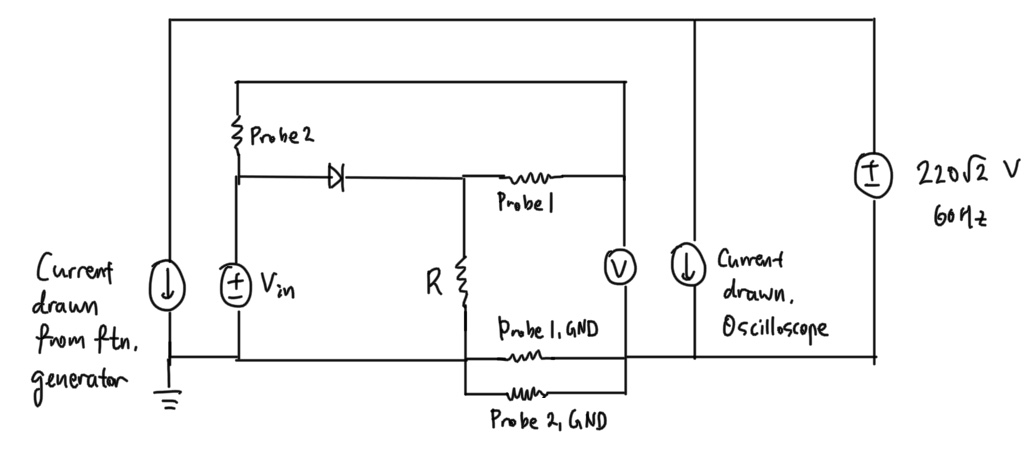
\includegraphics[width=0.5\linewidth]{Probe.jpeg}
    \caption{Reason of noise}
\end{figure}
As can be seen in Figure 1, because of the resistance in the probe wire($50$[m$\Omega$] range), and because of the current draw of the function generator and the oscilloscope from the wall outlet, any current in the $1$[A] range can create noise near the $50$[mV] range. As observed in table 1, the voltage across the resistor in reverse bias was $-40$[mV], and as observed in table 2, the max and min voltages are each about $40$[mV] higher than $\pm4$[V]. Also, in the image provided, the difference between $V_{in}$ and $V_{out}$ in the oscilloscope measuring the half wave rectifier showed a noise about $80$[mV](red waveform). Therefore, the reverse bias voltage in experiment 1 can be thought of as 0[V], and the max, min voltage of $V_{in}$ in experiment 2 can be thought of as $\pm4$[V].

If we calculate the $RC$ values again, using $V_p=4$[V] and maintaining other values, we get $C=0.339[\mu$F](90Hz), 0.341[$\mu$F](100Hz), 0.343[$\mu$F](110Hz), whereas $C=0.349[\mu$F](90Hz) when $V_p=4.043$[V]. Even a $40$[mV] change in voltage corresponds to $0.01[\mu$F] change in the capacitance, so combined with the error in the measurement of the capacitance, the results in experiment 2 do fit with theoretical expectations around $V_{d,on}=560$[mV].

Note that the difference between measured voltages are relatively free from noise, since they are subject to the same noise. That is why the difference in $V_{d,on}$ in each experiment ($720$[mV] in experiment 1, $563$[mV] in 90[Hz], $562$[mV] in 100[Hz], $526$[mV] in 110[Hz]) needs more explanation.
\subsubsection{Change of Diode Voltage due to Impedance}
\begin{center}
    \scalebox{0.6}{\begin{tikzpicture}
      \draw[->] (-3,0) -- (4.2,0) node[below] {$V_D$};
      \draw[->] (0,-1) -- (0,4.2) node[above] {$I_D$};
      \draw[scale=0.5,domain=-6:2.9,smooth,variable=\x, blue] plot ({\x},{0.5*(e^\x-1)}) node[right]{$I_D=I_S(\exp\dfrac{V_D}{V_T}-1)$};
      \draw[scale=1,domain=-2:4,smooth,variable=\x, red] plot ({\x},{-\x/2+2}) node[above]{$I_D=\dfrac{V_{in}-V_D}{R}$};
\end{tikzpicture}
}
\end{center}

The graph above shows that when impedance increases, the slope of the red line swings "downwards", while the intersection with the $V_D$ axis stays the same($=V_{in}$), therefore the intersection voltage(turn on voltage) decreases(imagine a door hinged at $V_D=V_{in}$, which swings lower as $R$ increases). Due to capacitance coupling and change of frequency, the equivalent impedance of the circuit changes, and thus $V_{d,on}$ changes, which is why we have to apply different values of $V_{d,on}$ for different circuits.

\end{document}
